\documentclass[doktyp=marbeit,fontsize=12pt,sprache=english,draft=true,hausschrift=true]{TUBAFarbeiten}

% packages
\usepackage{amsmath}
\usepackage[ngerman]{babel}
\usepackage{blindtext}
\usepackage{caption}
\usepackage{calc}
\usepackage{cite}
\usepackage{enumitem}
%\usepackage{float} % for better picture
\usepackage[T1]{fontenc}
\usepackage{floatrow} % rows of table and pictures
\usepackage{graphicx}
\usepackage{gensymb}
\usepackage[utf8]{inputenc}
\usepackage{makeidx}
\usepackage[fleqn]{mathtools} % mathtools und links buendig machen
\usepackage{multirow} % tabellen mit mehreren zeilen pro zelle
\usepackage{subcaption}
\usepackage{subscript} % tief stellen
%\usepackage[square]{natbib}
\usepackage{setspace}
\renewcommand{\baselinestretch}{1.5}

\DeclarePairedDelimiter{\abs}{\lVert}{\rVert} % definiere absoluten betrag

\usepackage[acronym,toc]{glossaries}
\glstoctrue%

\newglossary[nlg]{symbols}{nls}{nlo}{Symbol Definition}
\makeglossaries%

\newacronym{icp}{ICP}{Iterative Closest Points}
\newacronym{sift}{SIFT}{Scale Invariant Feature Transform}
\newacronym{surf}{SURF}{Speeded-Up Robust Features}

\newglossaryentry{bearing-angle}{%
    name={Bearing-Angle},
    description={The Bearing-Angle represents the angle betwen the lightray from the sensor to the depth value and the connection to a neighbouring depth value. The Bearing Angle can be calculated to arbitrary neighbouring depth values. Both laserscans and depth images can be converted using a proper intrinsic calibration of the sensors.},
    type=\acronymtype}

\newglossaryentry{bearing-angle-image}{%
    name={Bearing-Angle Image},
    description={The Bearing-Angle Image is a derived image type where each pixel encodes the Bearing-Angle for the lightray of this pixel. The angle is discretized from the range $(0, \pi)$ to the color depth of the target image. The resulting images are grayscale.},
    type=\acronymtype}

\newglossaryentry{flexion-image}{%
    name={Flexion Image},
    description={The Flexion Image is a way to convert range data.
    For each pixel of the depth image a scalar value that measures the angle between the estimated surface normals is computed and stored.
    This measure is useful for obtaining high-level image features from low-level geometry information.},
    type=\acronymtype}

\newglossaryentry{curvature}{%
    name={Curvature},
    description={Curvature is a concept from Differential Geometry that applies to manifolds. The principal curvatures $k_1$ and $k_2$ measure how surfaces bend at that point. Different specific types of curvature do exist.},
    type=\acronymtype}

\newglossaryentry{mean-curvature}{%
    name={Mean Curvature},
    description={Mean Curvature is the sum of $k_1$ and $k_2$ and of the main curvature types.},
    type=\acronymtype}

\newglossaryentry{gaussian-curvature}{%
    name={Gaussian Curvature},
    description={Gaussian Curvature is the product of $k_1$ and $k_2$ and is used in many fields. It gives the tool to classify points on a surface based onf sign and magnitude. For negative values of the Gaussian Curvature the point is said to be hyperbolic, for positive values the point is said to be an elliptic point. Points with Gaussian Curvature being zero are parabolic points.},
    type=\acronymtype}

\newglossaryentry{max-curve-image}{%
    name={Max-Curve Image},
    description={This image is a feature image, similar to \Glspl{bearing-angle-image}. For each pixel the sum of each \Gls{bearing-angle} in forward and backward direction is calculated. This angle is calculated in both diagonals, horizontal and vertical direction. Finally the maximum value is used as pixel value after scaling.},
    type=\acronymtype}

\newglossaryentry{Vectors}{%
    name={$\vec{v}$},
    description={mathematical vectors are written as small letters with arrow},
    type=symbols}


\input{thesis-metadata}

\setcounter{tocdepth}{2}
%\setcounter{secnumdepth}{3}

% \makeindex

% start the content
\begin{document}

\maketitle

\TUBAFErklaerungsseite%
\tableofcontents
\newpage

\printglossary[type=\acronymtype]%
\newpage

\printglossary[type=symbols]%
\glsaddallunused[symbols]
\newpage

% \newpage

\section{Proposal}

The dominant method to register pointclouds with pointclouds or depth
images is the use of a variant of the \gls{icp}\cite{Besl1992}
algorithm. Pomerleau et.al\cite{Pomerleau2015} provide a review of pointcloud registration methods.
Even though there are many different variations of \gls{icp}, it has
some common problems. The algorithm requires a good initial
transformation. Pointclouds with order-of-magnitude different
resolutions can produce unstable results. Convergence might require many
iterative steps and can not be predicted. Each of these iterative steps
is computationally expensive and does not scale very well to massive
datasets.

All these apsects give opportunity for a better solution to the problem
of registering depth images, e.g.~from the Kinect-v2, to existing
high-resolution pointclouds.
Inspired by Scaramuzza's \Glspl{bearing-angle-image}\cite{Scaramuzza2007}, Lin et.al\cite{Lin2017} apply the classical feature detector \gls{surf}\cite{Bay2006} on \Glspl{bearing-angle-image} and are able to register pointclouds to each other.
This work improves upon this idea in multiple ways.
\Glspl{bearing-angle-image} are not rotation invariant as they encode local geometry only in one direction.
Neither are they viewpoint invariant, as the \gls{bearing-angle} changes when the sensing lightray hits the same surface from a different angle.
In an attempt to overcome these limitations this work proposes new derived images that are rotation and viewpoint invariant, with the most promising variant being \Glspl{flexion-image}.

\subsection{Approach}\label{approach}

\subsubsection{Preprocessing of range Data}\label{preprocessing-of-range-data}

\begin{figure}[H]
    \centering
    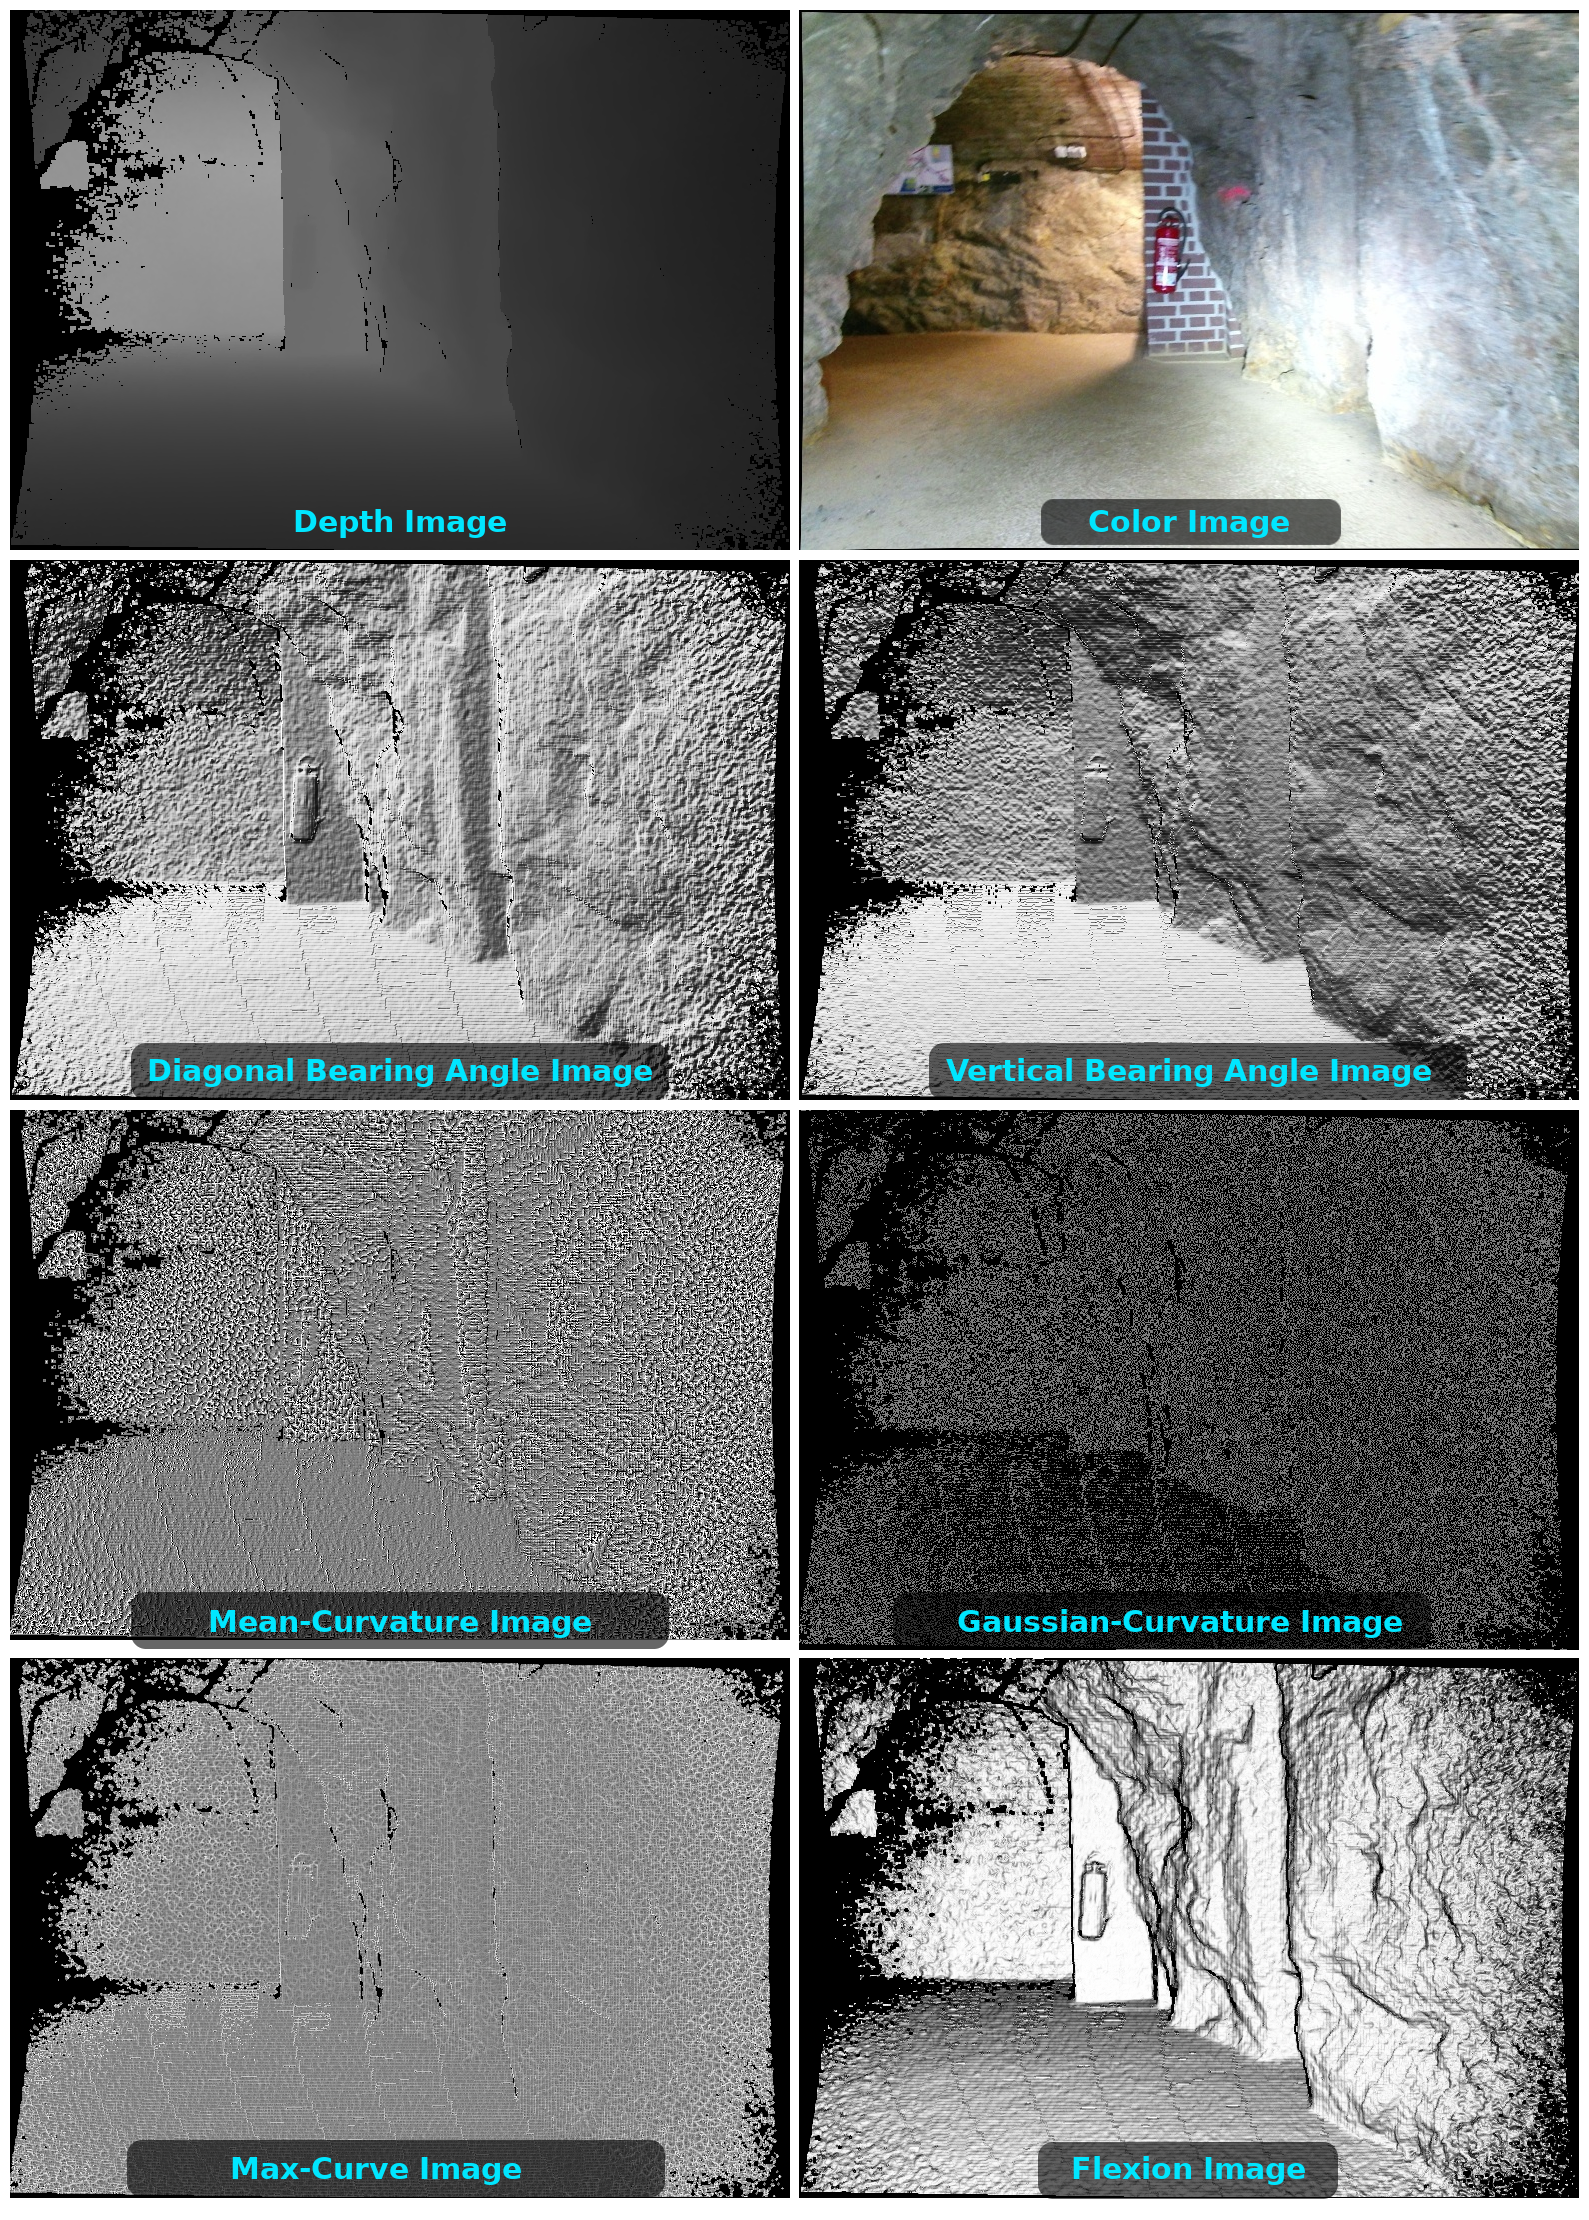
\includegraphics[width=0.9\textwidth]{images/collage_v3.png}
    \caption{Overview of possible Feature-Images from a depth image.}
\end{figure}

Instead of registering the depth images based on single points as \gls{icp} algorithms do, this thesis develops a new framework to use existing image features like \Gls{sift} and \Gls{surf} to calculate the transformation between pointcloud and depth image.
Both, the pointcloud and the depth image, are first converted to a gray-scale feature image.
Local geometric structure is encoded through the visual structure of the feature image and is detected and matched via a classical matching pipeline.

\subsubsection{\Glspl{bearing-angle-image}}

\begin{figure}[H]
    \centering
    \includegraphics[width=0.5\textwidth]{images/scetch_bearing.png}
    \caption{This figure shows the relationship of the light rays that form the \gls{bearing-angle}.}
\end{figure}

Existing literature\cite{Scaramuzza2007,Lin2017} proposes \Glspl{bearing-angle-image} were each pixel is the angle between the current point, the optical center and the previous point.
The neighbourhood relationship can be choosen arbitrarily resulting in four first-order \Glspl{bearing-angle-image}, horizontal, vertical, diagonal and antidiagonal.
The second variable is the direction the angle is calculted, e.g.~for horizontal images it can be calculated from left-to-right or right-to-left.
This does not exhibit new information, because the angle of the other direction is immediatly known from the fact that the sum of the angles is $180\degree$.
Nontheless, the direction must be defined to obtain stable visual features.

The formula for the \gls{bearing-angle} $\beta$ is derived with the cosine theorem.
\[
    \beta = \acos \frac{2 \rho_{i,j} \rho_{i,j} - 2 \rho_{i,j} \rho{i-1,j-1} \cos d\phi}{2 \rho_{i,j} \sqrt{\rho_{i,j} \rho_{i,j} + \rho{i-1,j-1} \rho{i-1,j-1} - 2 \rho_{i,j} \rho{i-1,j-1} \cos d\phi}}
\]

\subsubsection{\Glspl{flexion-image}}

Each pixel of a \Gls{flexion-image} is dot-product of the local normal
calculated from horizontal and vertical neighbouring pixel with the
normal calculated with the diagonal neighbours.

The dot-product then results in the angle between both of these vectors.
The smaller the dot-product gets, the higher is the local flexion of the
surface. This local property of the geometry then results in visual
features detectable with classical feature detectors and descriptors like
\Gls{sift} or \Gls{surf}.

\subsubsection{Other derived image types}

- \gls{curvature} from differential geometry, experimenting with \gls{gaussian-curvature} and \gls{mean-curvature}.
- Different calculation for angles from local geometry
- curvature
- max-curve

\subsubsection{Transformation calculation}\label{transformation-calculation}

Starting with the feature image, a visual localization pipeline is
established that works solely on omnidirectional data, thus is general
enough to utilize a wide range of sensors and camera models.

The full workflow of the pipeline is as follows:

\begin{enumerate}
\item Omnidirectional images are mapped onto a cubemap to reduce distortion,
  the feature images are calculated for both the data to localize,
  e.g.~Kinect depth image and the reference data, e.g.~terrestrial
  laserscans.
\item Visual Features are detected and matched between the sensor to
  localize and the reference data.
\item Classical RANSAC performs the stable calculation of the
  Essential matrix that is then decomposed into rotation and translation.
\item The resulting rotation and translation is optimized. The objective
  function is the distance of the detected features to the epipolar
  lines.
\item The unscaled translation is scaled with the depth data from the sensor
  input. This scaling can be done both with the input depth sensor and
  the reference data. The resulting difference is again subject to
  optimization.
\end{enumerate}

The result is the pose of the camera relative to the registered image as well as an error of the pose.

\subsection{Novelity}\label{novelity}

The idea to use optical features for multimodal sensor registration is
not new and goes back to Scaramuzza's approach to calibrate a
laserscanner to an optical camera. To the best knowledge of the author
only bearing angle images were used though.

Bearing angle images do come with some issues. They encode only the
relationship of two neighbouring points. Therefore, they are not
invariant to rotation. It is possible to calculate the bearing angle in
all eight bearing directions (horizontal, vertical, diagonal, antidiagonal in
both directions). This results to higher computational costs, especially
for the feature detection and matching pipeline.

This is the reason this work proposes different feature images that all
encode local geometry as a scalar value, gaussian curvature, mean
curvate and flexion as described above. These feature images are
compared to bearing angles. Flexion images are expected to perform the best
as they give the best visual structure.

If the proposed localization pipeline does work as wished it gives a new
intermodal approach to localization and visual odometry.

Futhermore, it allows to apply algorithms and approaches from the
classical visual feature-world to depth sensors that became widely
available in robotic operations.

% \input{verzeichnisse/bezeichnungen.tex}
% \newpage
%
% \input{einfuehrung/content.tex}
% \newpage
% \input{grundlagen/content.tex}
% \newpage
% \input{modelle/content.tex}
% \newpage
% \input{intrinsic/content.tex}
% \newpage
% \input{extrinsic/content.tex}
% \newpage
% \input{evaluierung/content.tex}
% \newpage
% \input{fazit/content.tex}
% \newpage

\begin{appendix}
    % \appendix
    % \input{anhang/content}
    \newpage

    \addcontentsline{toc}{section}{\bibname}
    \bibliographystyle{IEEEtran}
    \bibliography{references}

    \newpage
    \addcontentsline{toc}{section}{\listtablename}\listoftables

    \newpage
    \addcontentsline{toc}{section}{\listfigurename}\listoffigures
    % \newpage

    %\renewcommand{\indexname}{Stichwortverzeichnis}
    %\addcontentsline{toc}{section}{Stichwortverzeichnis}
    % \printindex
\end{appendix}

\end{document}
